\documentclass{EESD}

% Important packages to be called
\usepackage{subcaption} % for adding sub-figures
\usepackage{graphicx}
\usepackage{tikz} % for cool graphics and drawings

\usepackage[absolute,overlay]{textpos} % To place the figures by coordinates (x,y) - Beamer doesn't support floats XD
\usepackage{multicol} % To adjust items and stuff automatically in a number of a pre-specified columns
\graphicspath{{Figures}}
\usepackage[utf8]{inputenc}
\usepackage{amsmath}
\usepackage{amsfonts}
\usepackage{amssymb}
\usepackage{dblfloatfix}
\usepackage{hyperref}
% fonts packages
\usepackage{ragged2e} % Justified typesetting

% For References Only
\usepackage[style=authortitle,backend=bibtex]{biblatex}
\addbibresource{References.bib} % Call the references database
\AtBeginBibliography{\tiny} % Specify font size (Size matters)
\renewcommand{\footnotesize}{\tiny}

% For adding code blocks
\usepackage{listings}
\lstset
{
    language=[LaTeX]TeX,
    breaklines=true,
    basicstyle=\tt\scriptsize,
    keywordstyle=\color{blue},
    identifierstyle=\color{magenta},
    commentstyle=\color{red},
    rulecolor=\color{black},
    numbers=left,
    numberstyle=\tiny\color{black},
    % framexleftmargin=15pt,
    frame = single,
}


%%%%%%%%% Shortcuts
\newcommand{\x}{\ensuremath{h}}
\newcommand{\params}{\ensuremath{\boldsymbol{\theta}}}


\author{Hannah Plath, Thiago Petrilli Maffei Dardis, Alexandre Allauzen}
\title[AIAE'22]{Experimental study of Neural ODE training with adaptive solver for dynamical systems modeling}

\institute[ESPCI-PSL]{{ESPCI Paris - PSL}{\newline\newline MILES team – Université Paris Dauphine}}
\subject{}
\date{December 1st, 2022}

\begin{document}

{ % <-- don't forget the scope resolution (Brackets) to limit the background change only for the cover page; otherwise, it will override the whole document's background :)
\usebackgroundtemplate{} % To add a background for this slide XD - Empty one
\coverpage{
\titlepage{~}
% To add additional text to the title components 
}
} % <-- and yeah close them too :)


\setbeamertemplate{logo}{} % To override the logo from the other slides and delete it completely


% -----------------------Table of contents TOC Three Styles
% Explicitly split the TOC if it's too long
% \begin{frame}[allowframebreaks]{Outlines}
% \tableofcontents[sections={1-3}] % Explicitly split TOC
% \framebreak
% \tableofcontents[sections={4-7}] % Explicitly split TOC
% \end{frame}

% % Just a normal TOC 
% \begin{frame}[allowframebreaks]{Outlines}
% \tableofcontents
% \end{frame}

% Use smart division for the TOC
\begin{frame}{Outlines}
\begin{multicols}{2}
\tableofcontents
\end{multicols}
\end{frame}

% -----------------------Introduction
\section{Introduction}

\breakingframe{
\begin{textblock*}{3cm}[0.5,0.5](0.5\textwidth,  0.5\textheight)
\Huge\textbf{\textcolor{black}{Introduction}}
\end{textblock*}
}


\begin{frame}{From ResNet to Neural ODE}
  A deep Network is a cascade of $K$ transformations/layers , for the k$^{th}$ layer
  $$
  \x_k = { \color{red} \underbrace{\ \x_{k-1}\ \ +\ }_{
      \begin{array}{c}
        \text{Residual}\\
        \text{connexion}
      \end{array}
    } }
  \underbrace{\ f_{\params_k} (\x_{k-1}) \ }_{
    \begin{array}{c}
      \text{Neural-Net}\\
      \text{Layer}
    \end{array}
  }
  $$
  
  \begin{itemize}
  \item The residual connexion allows the model to be very deep 
  \item Help for the vanishing gradient issue
  \end{itemize}


  \begin{alertblock}{If $K \ \longrightarrow\ \infty$}
        $$\frac{dh(t)}{dt} = f(h(t), t, \params), \text{ the NNet is now a model of the dynamics}$$
  \end{alertblock}
  
\end{frame}

\subsection{Neural ODEs}
\begin{frame}[t]{Neural ODEs}
\begin{itemize}
    \item We can parameterize the continuous dynamics of hidden states in Neural Networks with an ODE:\vspace{10pt}
    \begin{equation}
        \frac{dh(t)}{dt} = f(h(t), t, \params) 
    \end{equation}\pause
    \item Starting from the input layer $h(0)$, we can define the output layer $h(T)$ to be the solution to this ODE initial value problem at some time $T$.\vspace{10pt}\pause
    \item From the hidden state $z(t_0)$ we can define the loss function at $z(t_1)$ as:
    \begin{equation}
        L(z(t_1)) = L(z(t_0)+\int_{t_0}^{t_1} f(z(t), t, \params))dt
    \end{equation}\vspace{10pt}
\end{itemize}
\end{frame}

\subsection{Lorenz’63}
\begin{frame}[t]{Lorenz’63}
\begin{itemize}
    \item This butterfly attractor is broadly used as a benchmark for time series modeling\pause
    \item Consider a point $x\in \mathcal{R}^3$ with its three coordinates $x_1$, $x_2$, $x_3$. The Lorenz’63 system consists of three coupled nonlinear ODEs:
    \begin{equation}
    \begin{aligned}
        &\dot{x_1} = \frac{dx_1}{dt} = \sigma(x_2 - x_1), \\ 
        &\dot{x_2} = x_1(\rho - x_3) - x_1, \\
        &\dot{x_3} = x_1 x_2 - \beta x_3
    \end{aligned}
    \end{equation}
    \vspace{10pt}\pause
    \item In this work we consider the standard setting ($\beta$ = 8/3, $\sigma$ = 10, $\rho$ = 28), such that the solution exhibits a \textit{chaotic} regime. \vspace{10pt}
\end{itemize}
\end{frame}

% -----------------------Fehlberg's Method

\section{Fehlberg's Method}
\breakingframe{
\begin{textblock*}{16cm}[0, 0](0.29\textwidth,  0.5\textheight)
\Huge\textbf{\textcolor{black}{Fehlberg's Method}}
\end{textblock*}
}

\subsection{Evaluations of $f_{\params}$}
\begin{frame}[t]{Evaluations of $f_{\params}$}
\begin{itemize}
    \item The method requires three evaluations of $f_{\params}$ for a fixed step-size $h$:
    \begin{equation}
        \begin{aligned}
            f_1 = f_{\params}(x_i),\ f_2 = f_{\params}(x_i + hf_i),\ f_3 = f_{\params}(x_i + \frac{h}{4}[f_1 + f_2])
        \end{aligned}
    \end{equation}\pause
    \item Then, we can compute two approximations for the next point:
    \begin{equation}
        \begin{aligned}
            A_1 = x_i + \frac{h}{2}[f_1 +f_2]\ (RK2\ method), and A_2 = x_i + \frac{h}{6}[f_1 + f_2 + 4f_3]\ (RK3)
        \end{aligned}
    \end{equation}\vspace{10pt}\pause
    \item Then, we can estimate the following error:
    \begin{equation}
        \begin{aligned}
            r = \frac{|A_1 - A_2|}{h} \simeq Kh^2
        \end{aligned}
    \end{equation}\vspace{10pt}
\end{itemize}
\end{frame}

\begin{frame}[t]{Evaluations of $f_{\params}$}
\begin{itemize}
    \item If $r>\epsilon$, then $A_2$ is rejected and we need to restart the computation with \begin{equation}
        h'= S \times h\sqrt{\epsilon/r}
    \end{equation}\pause
    \item We've used the following default values: $h$=1, $S$=0.9 and $\epsilon$=0.1.
\end{itemize}
\end{frame}


% -----------------------Experiments
\section{Experiments}
\breakingframe{
    \begin{textblock*}{5cm}[0.3,0.5](0.5\textwidth, 0.5\textheight)
        \textbf{\Huge{Experiments}}
    \end{textblock*}
}

\subsection{Trajectories prediction}
\begin{frame}{Trajectories prediction}
    \begin{figure}
        \centering
        \hspace*{-1.5cm}
        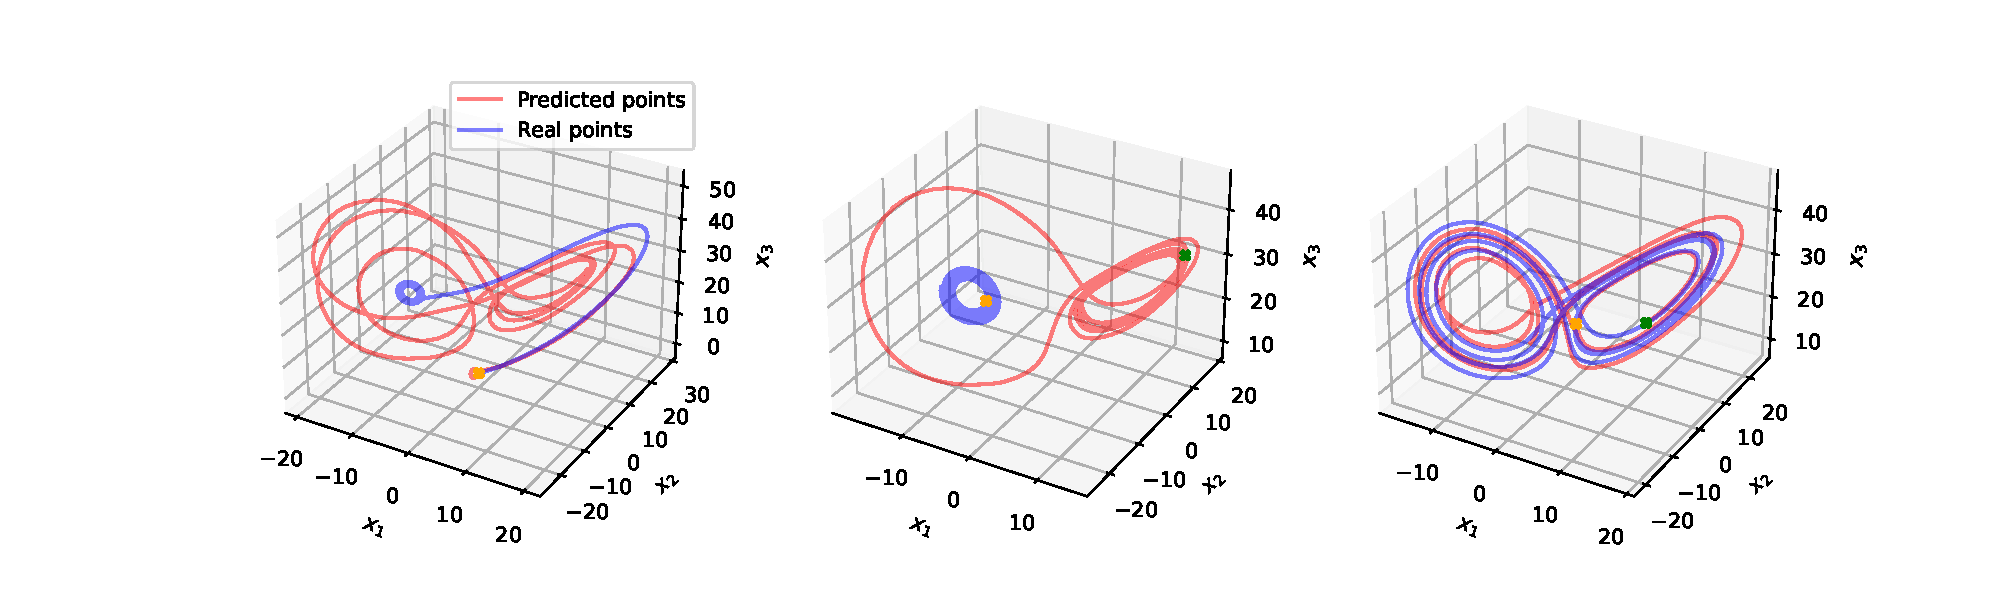
\includegraphics[width=16cm]{baseline_lorenz_3}
        \caption{Each figure depicts a different time slice of the
          generated trajectory and of the original training data: from
          0 to 600, 600 to 1200 and 2000 to 2600.}
        \label{fig:lorenz}
    \end{figure}
\end{frame}


\subsection{Performance}
\begin{frame}{Performance}
    \begin{figure}
        \centering
        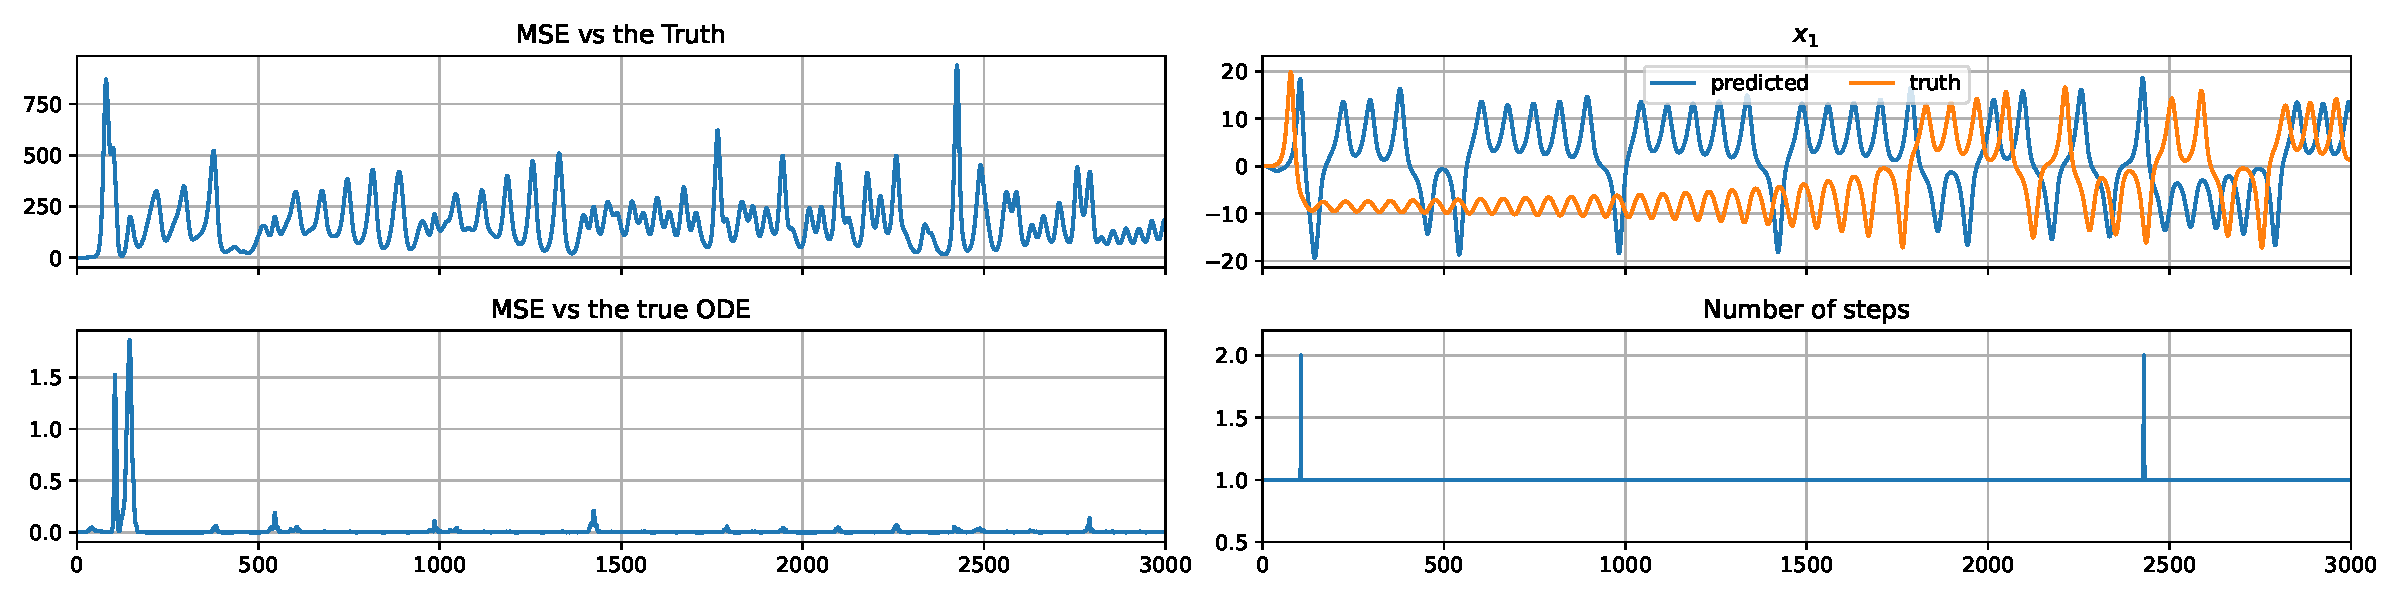
\includegraphics[width=14cm, height=5cm]{baseline_time_series_2x2}
        \caption{Time evolution of (from left to right and top to bottom): the MSE, the evolution of $x_1$, the MSE w.r.t the true ODE of Lorenz’63, and the number of steps.}
        \label{fig:lorenz_error}
    \end{figure}                                                    
\end{frame}

\section{Fehlberg's Training}
\breakingframe{
    \begin{textblock*}{16cm}[0, 0](0.29\textwidth,  0.5\textheight)
        \textbf{\Huge{Fehlberg's Training}}
    \end{textblock*}
}

\subsection{Results}
\begin{frame}{Results}
    \begin{figure}
        \centering
        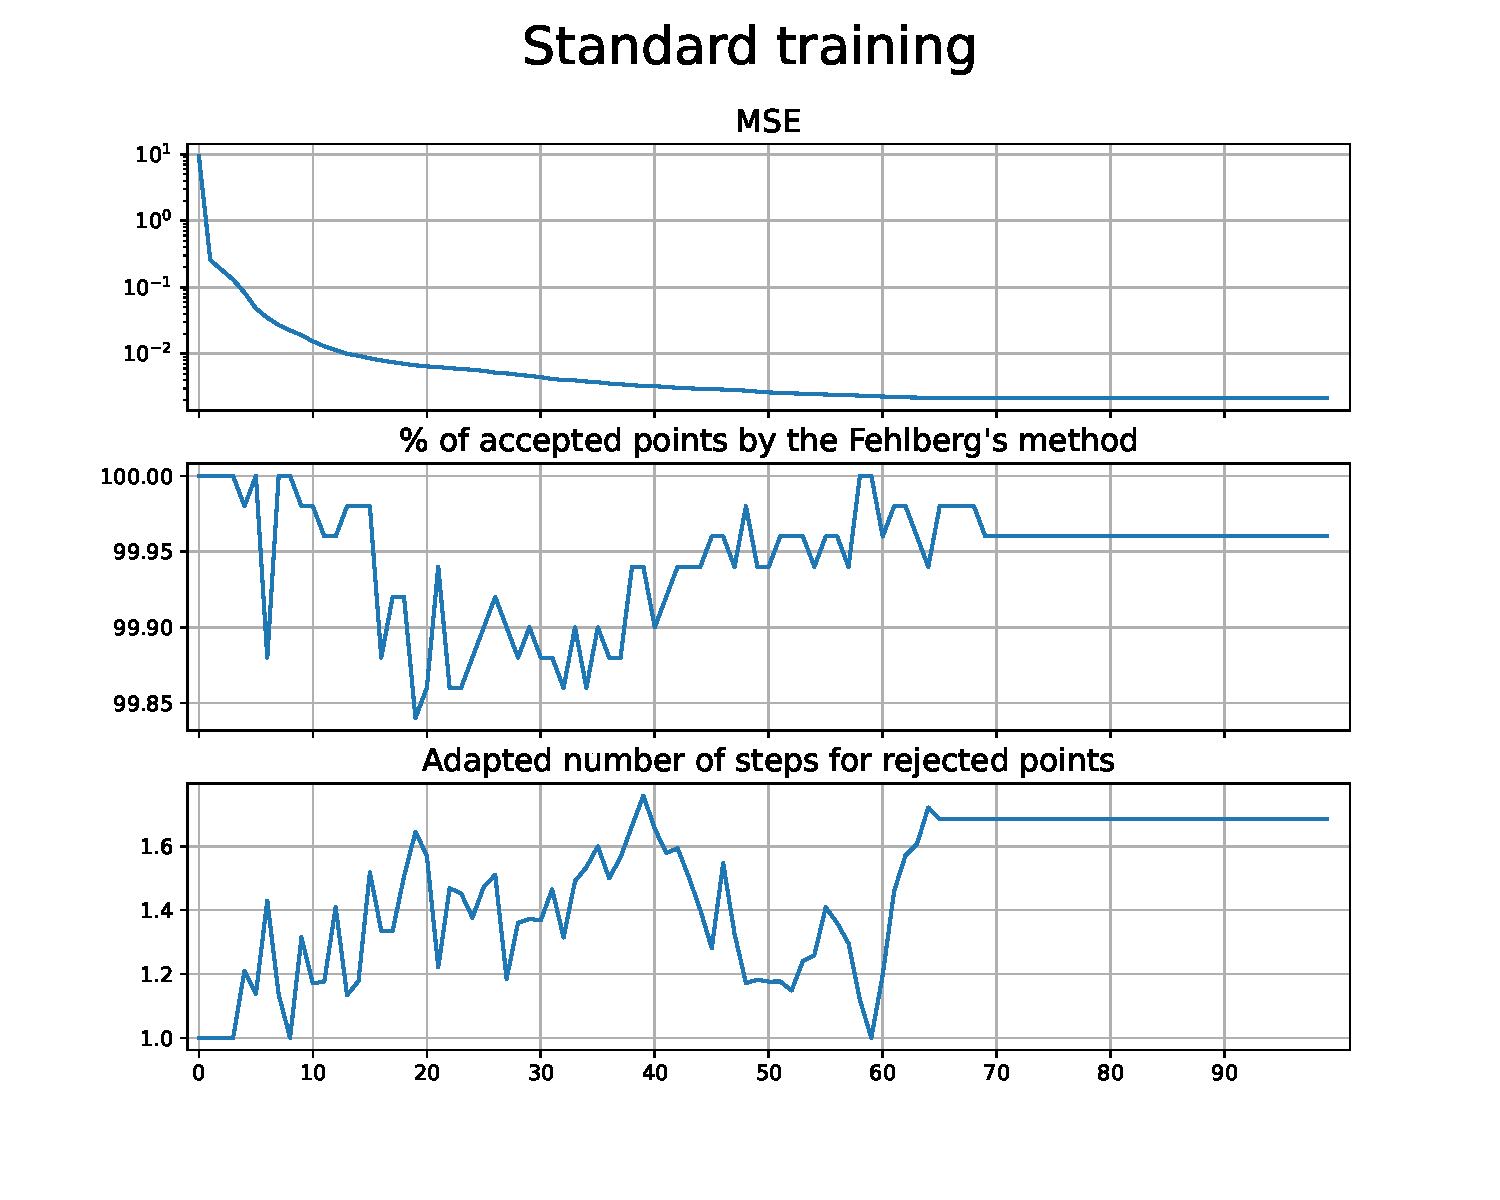
\includegraphics[width=0.49\textwidth]{batch_training.pdf}
        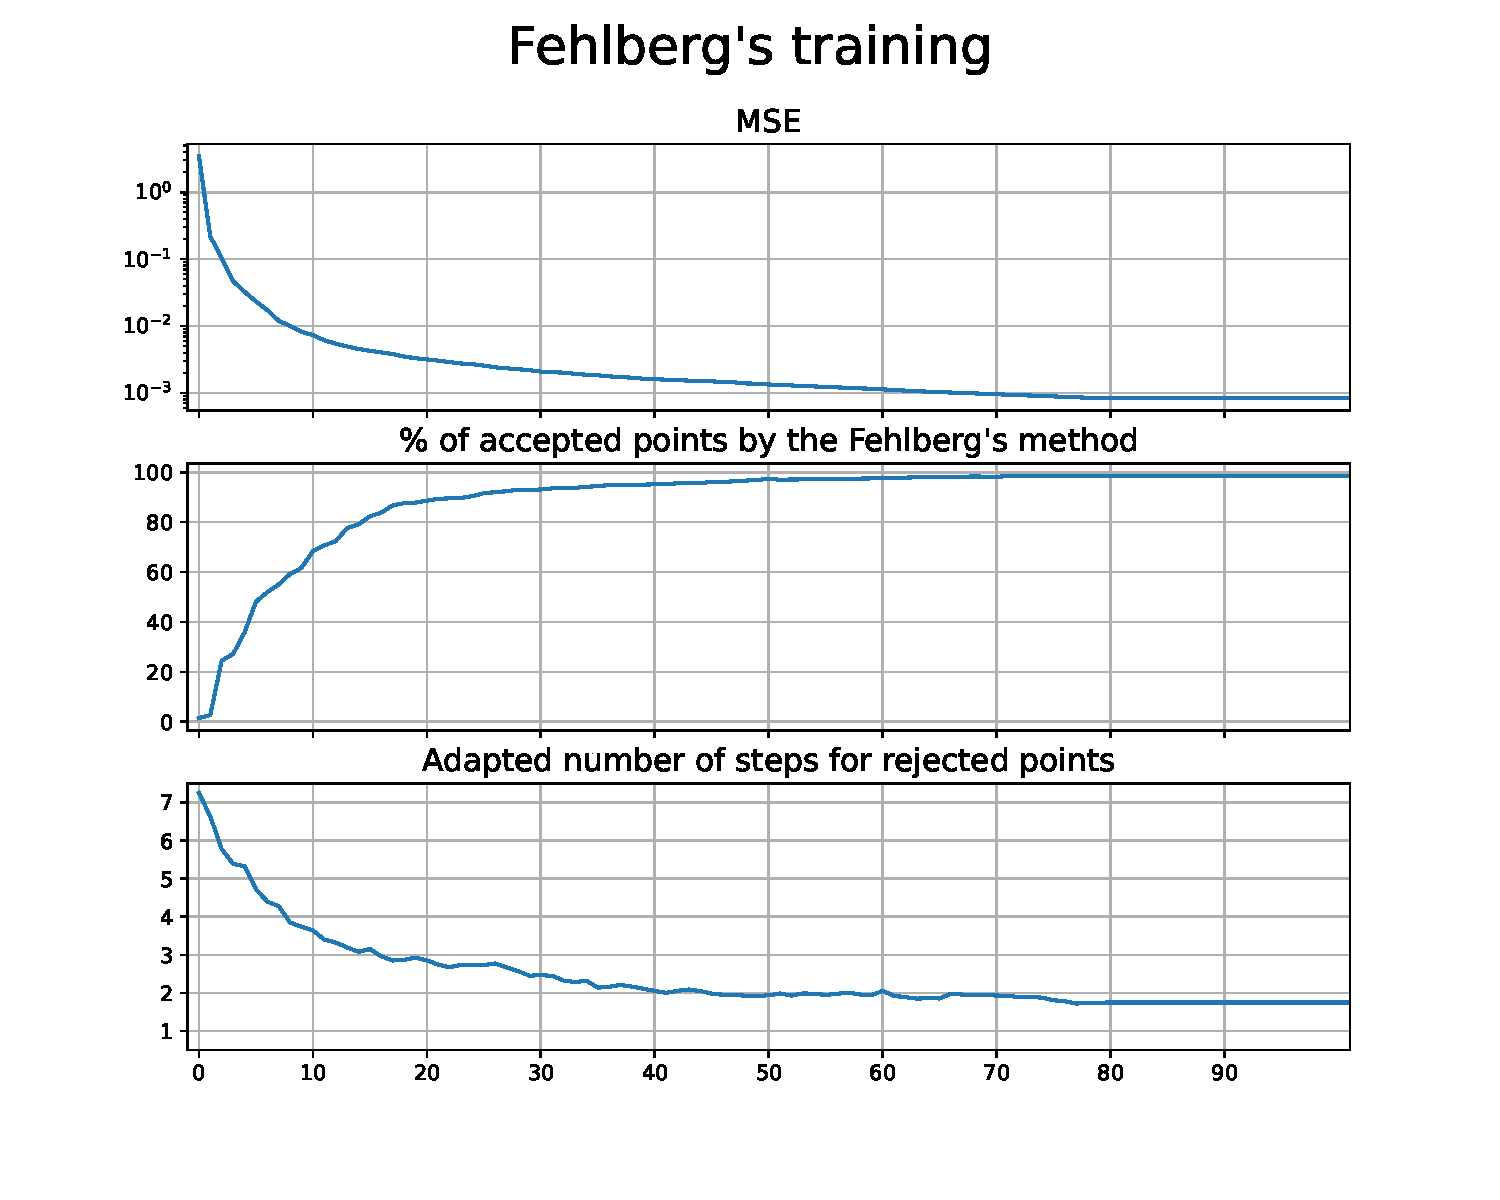
\includegraphics[width=0.49\textwidth]{fehlberg_training.pdf}
        \caption{Time evolution for two training conditions of: the MSE loss; the percentage of accepted hypotheses $A_2$; the new number of steps for the rejected hypotheses (before rounding).}
        \label{fig:lorenz_error}
    \end{figure}                                                    
\end{frame}


\section{Conclusion}
\breakingframe{
    \begin{textblock*}{16cm}[0, 0](0.29\textwidth,  0.5\textheight)
        \textbf{\Huge{Conclusion}}
    \end{textblock*}
}

\begin{frame}{Take-home message: whatch your step size !}
  \begin{itemize}
  \item Neural \textbf{ODE} relies on
    solvers for inference and training. 
  \item  Adaptive solvers cannot be seamlessly
    leveraged as a black-box: % for dynamical systems modelling.
  \end{itemize}
  \begin{alertblock}{Our contributions:}
    \begin{itemize}
    \item[$\rightarrow$] For most of the numerical methods, the step size is adapted given the self-estimated error of the model.
    \item[$\rightarrow$] Neural ODE model is always self-confident, and the ``adaptive'' ability is under-used. 
    \item[$\rightarrow$] A simple workaround:
    \end{itemize}
  \begin{center}
    use the supervision within the solver.
  \end{center}
      \hfill\url{https://github.com/Allauzen/adaptive-step-size-neural-ode}
  \end{alertblock}
\end{frame}

% -----------------------References
% Thank you slide should be here
\breakingframe{
\begin{textblock*}{15cm}(1.8cm,4cm)
\Huge\textbf{\textcolor{black}{Thank you for your attention!}}
\end{textblock*}
}


\breakingframe{
\begin{figure}
    \centering
    \vspace{1.3cm}
    
\includegraphics[width=0.3\textwidth]{qrcode.png}
\end{figure}
}

\end{document}
